\documentclass[tikz,border=2mm,background=white]{standalone}
\usepackage{tikz}
\usetikzlibrary{matrix,arrows.meta,positioning,backgrounds}

\tikzset{
  level0/.style={rectangle, draw=black, fill=magenta!30, font=\bfseries\large, minimum width=2cm, minimum height=1cm},
  level1/.style={rectangle, draw=black, fill=green!50!white, font=\bfseries\large, minimum width=2cm, minimum height=1cm},
  level2/.style={rectangle, draw=black, fill=blue!40!white, font=\bfseries\large, minimum width=2cm, minimum height=1cm},
  level3/.style={rectangle, draw=black, fill=orange!40!white, font=\bfseries\large, minimum width=2cm, minimum height=1cm},
  newOp/.style={line width=2pt}
}

\begin{document}
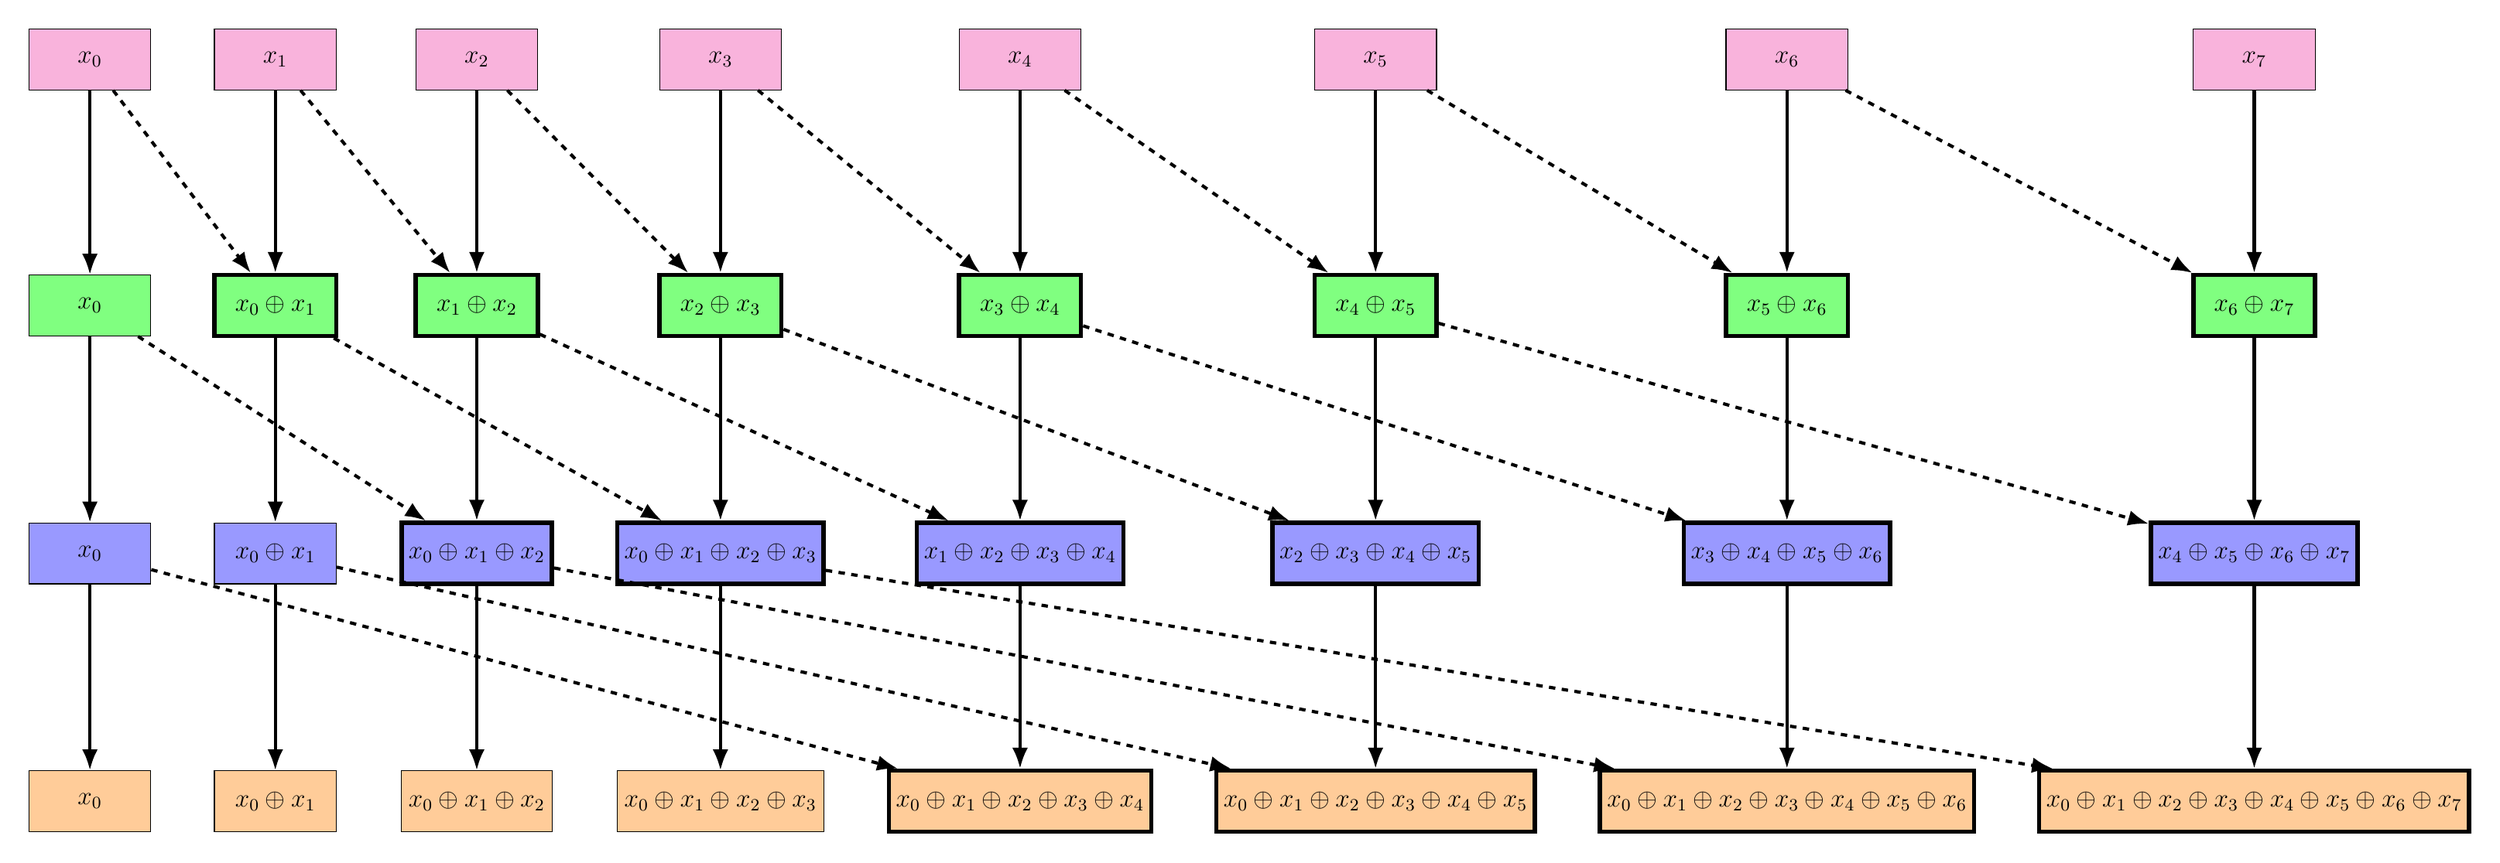
\begin{tikzpicture}[>=Latex]

% Matrix to force vertical alignment
\matrix[column sep=1cm, row sep=3cm] (m) {
  % Level 0
  \node[level0] (A0) {$x_0$}; &
  \node[level0] (A1) {$x_1$}; &
  \node[level0] (A2) {$x_2$}; &
  \node[level0] (A3) {$x_3$}; &
  \node[level0] (A4) {$x_4$}; &
  \node[level0] (A5) {$x_5$}; &
  \node[level0] (A6) {$x_6$}; &
  \node[level0] (A7) {$x_7$}; \\
  % Level 1
  \node[level1] (B0) {$x_0$}; &
  \node[level1,newOp] (B1) {$x_0 \oplus x_1$}; &
  \node[level1,newOp] (B2) {$x_1 \oplus x_2$}; &
  \node[level1,newOp] (B3) {$x_2 \oplus x_3$}; &
  \node[level1,newOp] (B4) {$x_3 \oplus x_4$}; &
  \node[level1,newOp] (B5) {$x_4 \oplus x_5$}; &
  \node[level1,newOp] (B6) {$x_5 \oplus x_6$}; &
  \node[level1,newOp] (B7) {$x_6 \oplus x_7$}; \\
  % Level 2
  \node[level2] (C0) {$x_0$}; &
  \node[level2] (C1) {$x_0 \oplus x_1$}; &
  \node[level2,newOp] (C2) {$x_0 \oplus x_1 \oplus x_2$}; &
  \node[level2,newOp] (C3) {$x_0 \oplus x_1 \oplus x_2 \oplus x_3$}; &
  \node[level2,newOp] (C4) {$x_1 \oplus x_2 \oplus x_3 \oplus x_4$}; &
  \node[level2,newOp] (C5) {$x_2 \oplus x_3 \oplus x_4 \oplus x_5$}; &
  \node[level2,newOp] (C6) {$x_3 \oplus x_4 \oplus x_5 \oplus x_6$}; &
  \node[level2,newOp] (C7) {$x_4 \oplus x_5 \oplus x_6 \oplus x_7$}; \\
  % Level 3
  \node[level3] (D0) {$x_0$}; &
  \node[level3] (D1) {$x_0 \oplus x_1$}; &
  \node[level3] (D2) {$x_0 \oplus x_1 \oplus x_2$}; &
  \node[level3] (D3) {$x_0 \oplus x_1 \oplus x_2 \oplus x_3$}; &
  \node[level3,newOp] (D4) {$x_0 \oplus x_1 \oplus x_2 \oplus x_3 \oplus x_4$}; &
  \node[level3,newOp] (D5) {$x_0 \oplus x_1 \oplus x_2 \oplus x_3 \oplus x_4 \oplus x_5$}; &
  \node[level3,newOp] (D6) {$x_0 \oplus x_1 \oplus x_2 \oplus x_3 \oplus x_4 \oplus x_5 \oplus x_6$}; &
  \node[level3,newOp] (D7) {$x_0 \oplus x_1 \oplus x_2 \oplus x_3 \oplus x_4 \oplus x_5 \oplus x_6 \oplus x_7$}; \\
};

% Draw arrows
\foreach \i in {0,...,7} {
  \draw[->, line width=1.5pt] (A\i) -- (B\i);
  \draw[->, line width=1.5pt] (B\i) -- (C\i);
  \draw[->, line width=1.5pt] (C\i) -- (D\i);
}

% Draw skip arrows (dashed with arrowheads)
\foreach \i/\j in {0/1,1/2,2/3,3/4,4/5,5/6,6/7} {
  \draw[->, dashed, line width=1.5pt] (A\i) -- (B\j);
}
\foreach \i/\j in {0/2,1/3,2/4,3/5,4/6,5/7} {
  \draw[->, dashed, line width=1.5pt] (B\i) -- (C\j);
}
\foreach \i/\j in {0/4,1/5,2/6,3/7} {
  \draw[->, dashed, line width=1.5pt] (C\i) -- (D\j);
}


\end{tikzpicture}
\end{document}
